
\documentclass[aspectratio=1610, 13pt]{beamer}
\usepackage{ctex}
\usepackage{CJKutf8}
\usepackage{xcolor}
\usepackage{multicol}
\usepackage{mathtools,array}
\usepackage[T1]{fontenc}
\usepackage{zi4}
\usepackage[font={scriptsize,bf}]{caption}
% \usepackage{subcaption}
\usepackage{graphics}
\usepackage{tikz}
\usepackage{fontawesome5}
\usepackage{mathpartir}

\newcommand{\naturals}{\mathbb{N}}
\newcommand{\reals}{\mathbb{R}}

\newcommand{\Dist}[1]{\mathcal{D}(#1)}
\newcommand{\expectation}{\mathbb{E}}

\newcommand{\states}{S}
\newcommand{\actions}{A}
\newcommand{\observables}{O}
\newcommand{\trans}{T}
\newcommand{\obs}{Z}
\newcommand{\reward}{R}
\newcommand{\discount}{\gamma}

\newcommand{\beliefs}{\mathcal{B}}
\newcommand{\beliefUpdate}{\tau}

\newcommand{\policy}{\pi}

\newcommand{\diff}[1]{\mathop{}\!\mathrm{d}#1}
\renewcommand{\figurename}{Figure}
\renewcommand{\refname}{Reference}

\AtBeginDocument{
  \catcode`_=12
  \begingroup\lccode`~=`_
  \lowercase{\endgroup\let~}\sb
  \mathcode`_="8000
}

% \usetheme{Madrid}
% % \usetheme{default}
% \setbeamertemplate{caption}[numbered]
% \setbeamerfont{title}{size=\large}
\mode<presentation>
{
  \usetheme{Darmstadt}      % or try Darmstadt, Madrid, Warsaw, ...
  \usecolortheme{default} % or try albatross, beaver, crane, ...
  \usefonttheme[onlymath]{serif}  % or try serif, structurebold, ...
  \setbeamertemplate{navigation symbols}{}
  \setbeamertemplate{caption}[numbered]
  \setbeamertemplate{footline}[frame number] 
} 

\usepackage{listings}
\lstdefinestyle{heaplang}{
    language=C,
    basicstyle=\footnotesize\ttfamily,
    keywordstyle=\color{blue},
    commentstyle=\color{red},
    escapeinside={<@}{@>},
    morekeywords={new_chan, fork, recv, send, swap, ref}
}
\lstdefinestyle{clang}{
    language=C,
    basicstyle=\footnotesize\ttfamily,
    keywordstyle=\color{blue},
    commentstyle=\color{red},
    escapeinside={<@}{@>},
}
\lstset{style=heaplang}

\usepackage{natbib}

\newcommand{\buchi}{B\"uchi }

\definecolor{goldenpoppy}{rgb}{0.99, 0.76, 0.0}
\definecolor{goldenyellow}{rgb}{1.0, 0.87, 0.0}
\definecolor{green2}{rgb}{0.1,0.7,0.3} 
\newcommand{\gcheck}{{\color{green2}\faCheckCircle[regular] }}
\newcommand{\rcross}{{\color{red} \faTimesCircle[regular]} }
\newcommand{\rflag}{{\color{red} \faFlag}}
% \usepackage{algorithm,amsmath}
% \usepackage[noend]{algpseudocode}

\newcommand{\zlstinline}{\let\par\endgraf\lstinline}
\newcommand{\comments}[1]{{\color{red}#1}}
\title{Group Meeting}
\date{\today}
\author{Members: Yong Li, Depeng Liu, Weizhi Feng, Xie Li, Shizhen Yu, Yutian Zhu, Zongxin Liu}
\begin{document}
\maketitle

\begin{frame}\frametitle{差分隐私——刘德鹏}
这周:
\begin{itemize}
  \item Pufferfish 杂志:基于POPL文章修改,当时对比CCS' 18的测试工具,不知是否加入新工具的比较(20年的新工具扩展性强,但没有处理离散机制,比较可能不占优势);
  \item 读完 Proving that Programs Are Differentially Private (APLAS '19):加入任一噪声机制后,
  攻击者猜测的损失函数值比起不加扰动时反而变小,即更加能猜出原secret的值,有点不合常理;
  初步原因在于攻击者知道数据分布、所加机制、以及观察对应的数据分布,发现反例不符仍需进一步证明;
  \item 参加讨论班,阅读cav文章报告。
\end{itemize}

计划:
\begin{itemize}
  \item Pufferfish期刊整理投稿,新实验?期刊未定(FAC, I\&C等..);
  \item 继续研究文章中的问题,与隐私参数选取,utility有关;
  \item DP模型:RL相关model free/ model learning内容学习。
\end{itemize}
\end{frame}

\begin{frame}\frametitle{内存安全}
本周:
\begin{itemize}
\item 继续对函数调用的符号执行进行Debug,能跑通一个函数调用的例子。
\item 阅读 Principles of Program Analysis,进行了报告和讨论。
\item CAV报告分享。
\item 其他事务性工作。
\end{itemize}


TODO:
\begin{itemize}
\item 根据SV-COMP加入库函数语义的支持。
\item 代码的重构。
\item 继续跑例子进行测试和Debug。
\item 下周三报告以及其他文献阅读和调研。
\end{itemize}



\end{frame}
\begin{frame}{冯维直}
    \begin{itemize}
        \item 期刊文章:
        \begin{itemize}
            \item [-] 上周计划是将SDBA取补算法正确性证明写完,然后增加一个determinization (确定化,给定SDBA, 构建一个DRA) 的章节,目前完成进度:没有写完证明,但是增加了一些intuition和定义,方便证明里面叙述更清楚;determinization部分把构造写了,但是还没有写证明.
            \item [-] 实验部分之前做了一些简单实验,现在和Andrea一起对更多自动机的例子进行实验,和Andrea讨论用那些工具和命令进行比较,输入的benchmark中自动机的形式等.
        \end{itemize}
        \item 阅读
        \begin{itemize}
            \item [-] 看视频读CAV文章:1. 决策树学习生成ranking function这篇进行了报告;2.另一篇是用decoupled search做composed \buchi automata 的liveness verification, 感觉难一点,看了一部分,还没看懂. 
        \end{itemize}
        \item 计划
        \begin{itemize}
            \item [-] 期刊文章第6章写完,和Andrea继续做实验,根据实验情况开始写第七章.
            \item [-] 没读懂的CAV文章继续读完.
        \end{itemize}
\end{itemize}    
\end{frame}

\begin{frame}{Shizhen Yu}
进展:
    \begin{itemize}
        \item 上周略读了一篇CAV文章《 Reflections on Termination of Linear
        Loops》 ,已经分享过一个简单版本
        \item 正在读李老师安排我读的一篇DBA active learning的文章《 Learning Deterministic Automata on InfiniteWords》,尽量这周读完与李老师讨论
        
        \item 计划:
        \begin{itemize}
            \item [-] 精读一下 《 Reflections on Termination of Linear        Loops》 主要是看一下文章中几个结果的证明
            \item [-] 跟进一下静态分析讨论班的进度,补一下已经讲过的 《 Principles of Program Analysis》章节
            
        \end{itemize}
\end{itemize}    
\end{frame}

\begin{frame}\frametitle{朱雨田}
\begin{center}
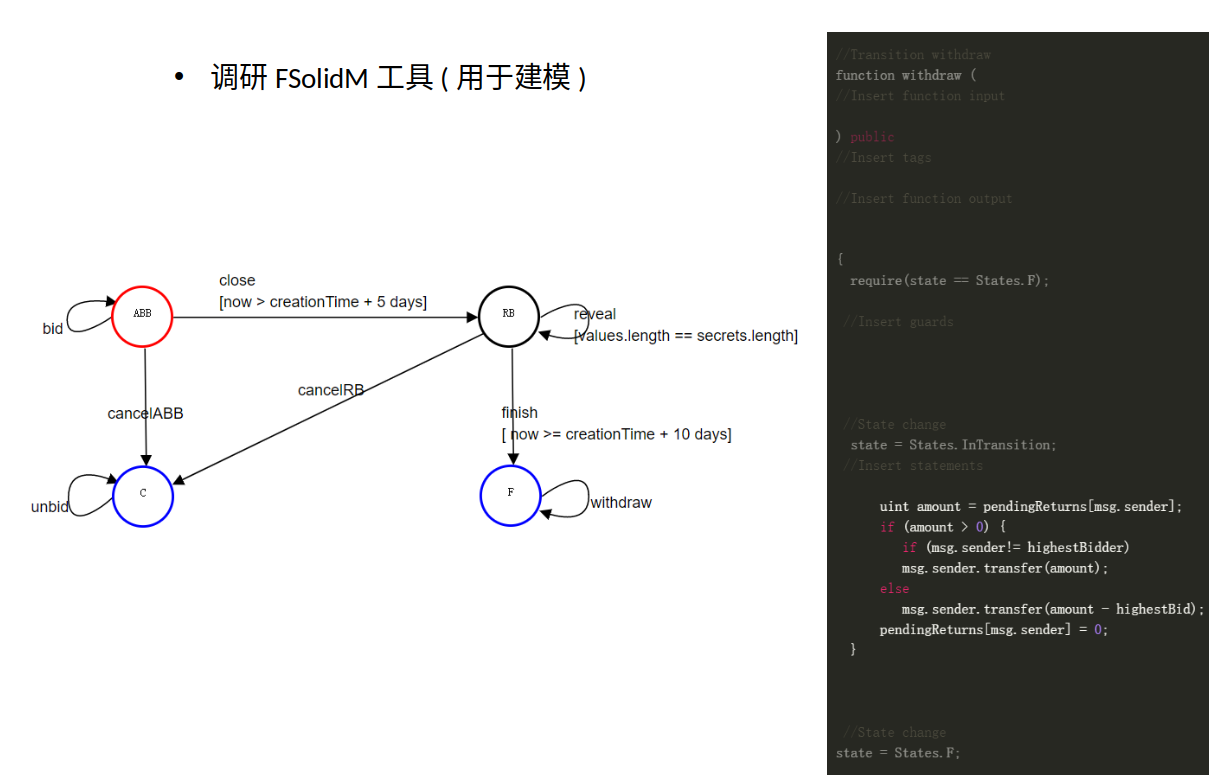
\includegraphics[scale=0.3]{zyt1.png}
\end{center}
\end{frame}

\begin{frame}\frametitle{朱雨田}
\begin{center}
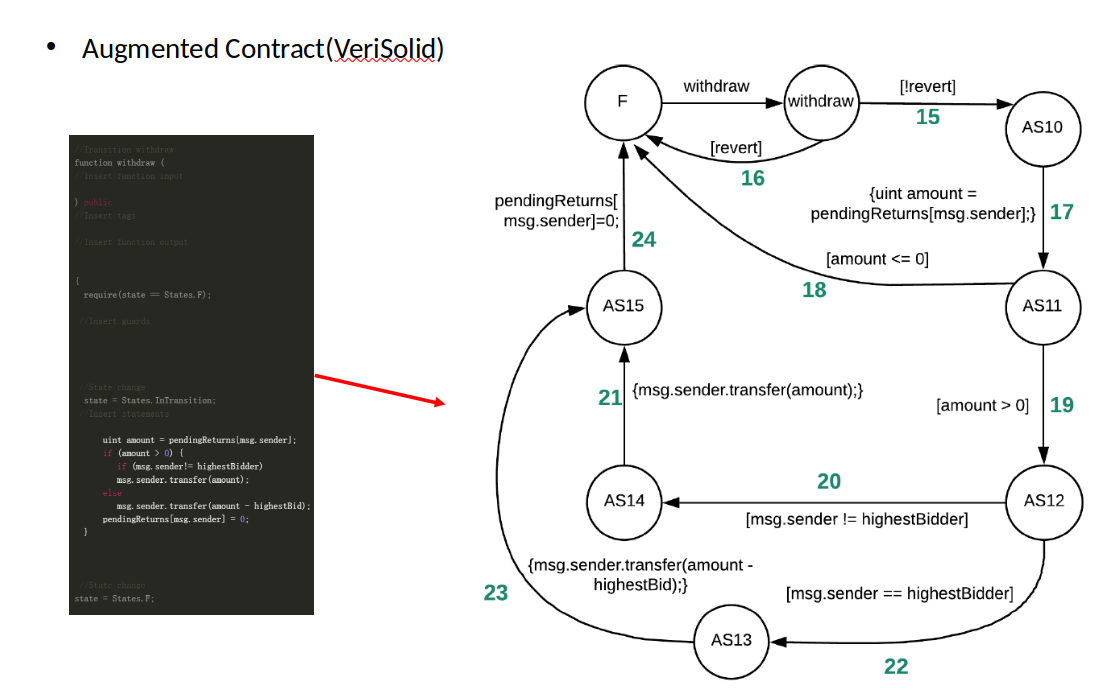
\includegraphics[scale=0.3]{zyt2.png}
\end{center}
\end{frame}

\begin{frame}\frametitle{朱雨田}
\begin{itemize}
\item 与锦龙师兄讨论了重用去年协议工程自动机建模部分的可行性。发现与FSolidM基本一致。
\end{itemize}
Plan:
\begin{itemize}
\item 继续调研VeriSolid,考虑用自动机对智能合约建模的具体做法(方案)。
\item 学习Solidity相关内容。
\item 继续阅读memory repair相关文章(option)。
\end{itemize}
\end{frame}

\end{document}